\chapter{Funzionalità} 

Le funzionalità messe a disposizione dall'applicazione \textit{PAO} sono:

\begin{itemize}
	\item \textit{\textbf{Aggiunta $\backslash$ Rimozione $\backslash$ Modifica}}: Di proprietari e animali sfruttando le peculiarità di \textit{QMap}. Ogni modifica avverrà tramite un inserimento di nuovi valori utilizzando la stessa chiave. Dal punto di vista grafico però non è il massimo.
	\item \textit{\textbf{PaoContainer}}: Il contenitore, già descritto in precedenza. Permette la modifica, l'aggiunta e la rimozione di Visite.
	\item \textit{\textbf{Encryption}}: Ogni classe \textit{AbstractOwner} ha un campo di tipo \textit{OwnerAccount} che a sua volta memorizza un \textit{QCryptographicHash} che rappresenta l'hash della password di un utente. La classe è pronta all'uso, in vista di future evoluzioni del software che potranno includere una schermata di login e un lato client.
	\item \textit{\textbf{Salvataggio su file}}: Tramite apposite funzioni, viene aperto un file in sola scrittura per ogni tipo di entità principale (Owner, Animal e Visit), viene allocato un \textit{QJsonObject} principale e successivamente, viene creato un \textit{QJsonArray} di \textit{QJsonObject}. \\ Per ogni elemento dei contenitori, vengono invocati i metodi \textit{save} dei singoli oggetti definiti nelle varie classi. Il contenuto viene quindi riversato nell'array ed infine, tramite il metodo \textit{write} di \textit{QJsonDocument}, viene effettuata la scrittura vera e propria su file.  
	\item \textit{\textbf{Caricamento da file}}: Viene fatto il processo opposto a quello di salvataggio, leggendo dai file scritti in precedenza tramite l'invocazione di apposite funzioni e i costruttori \textit{JSON} dei vari oggetti. Per implementare il tutto si è fatto uso della documentazione \textit{Qt} online. Un esempio di documentazione utilizzata è reperibile a fondo pagina \footnotetext[5]{ \url{https://doc.qt.io/qt-5/qtcore-json-savegame-example.html}}.
\end{itemize} 

\section{Interfaccia Grafica (GUI)}

Per la parte di interfaccia grafica si è cercato di dividere quanto più possibile la parte logica che interagisce con il database (il model) dalla parte grafica vera e propria (la view), secondo un pattern \textit{MVC}.\\ Per implementare questo pattern si è preferito creare due classi principali, descritte di seguito, piuttosto che avvalersi del MVC stile \textit{Qt} anche se quest'ultimo avrebbe garantito maggior riusabilità del codice e risultati migliori. 
Le due classi sviluppate sono:

\begin{itemize}
	\item \textit{\textbf{vetcontrol}}: Interagisce col database, predisponendo gli elementi nella tabella e richiamando i metodi di inserimento, modifica e rimozione di elementi. Apre inoltre i pannelli per l'inserimento e la modifica di nuovi elementi. \\Si è pensato di generare i nuovi pannelli all'interno del controller, anche se sarebbe stata una cosa prettamente di competenza della view, in quanto questi ultimi interagiscono anche loro col database sottostante. 
	\item \textit{\textbf{vetview}}: La vista amministrativa principale. Questa vista è divisa in tre sezioni tramite cinque \textit{QGroupBox}. \\A sinistra abbiamo i pulsanti per aprire i pannelli di inserimento, a destra, dinamicamente, viene visualizzato uno dei tre \textit{QGroupBox} per modifica e rimozione (in base al valore della \textit{QComboBox} presente nel \textit{Widget} centrale)  e al centro abbiamo, oltre alla già menzionata \textit{QComboBox}, un \textit{QTableWidget} e un \textit{QPushButton} d'uscita. \\Una funzione principale prepara la GUI, impostando i vari elementi grafici e un'altra imposta le \textit{connect} per associare tra loro vari eventi secondo il sistema di \textit{signal} e \textit{slot} fornito dal framework \textit{Qt}. \\La maggior parte dei metodi di questa classe, sono metodi privati, non accessibili all'esterno della stessa. 
\end{itemize}

Rimangono quattro classi che implementano i pannelli di inserimento e quello di modifica.
\begin{itemize}
	\item \textit{\textbf{AddOwnerDialog}}: Permette l'inserimento di proprietari. Delle \textit{QLineEdit} permettono all'utente di inserire i vari dati, uno slot pubblico si occuperà al momento del salvataggio di fare un minimo di controlli, creare un \textit{Owner} e aggiungerlo alla mappa del database passando attraverso il controller.
	\item \textit{\textbf{AddAnimalDialog}}: Analoga a \textit{AddOwnerDialog}
	\item \textit{\textbf{AddVisitDialog}}: Analoga a \textit{AddOwnerDialog} e a \textit{AddAnimalDialog}
	\item \textit{\textbf{EditVisitDialog}}:Permette la modifica di una visita selezionata. E' lo stesso pannello di inserimento, riadattato per disabilitare alcune componenti grafiche.
\end{itemize}

\begin{figure}[H]
	\centering
	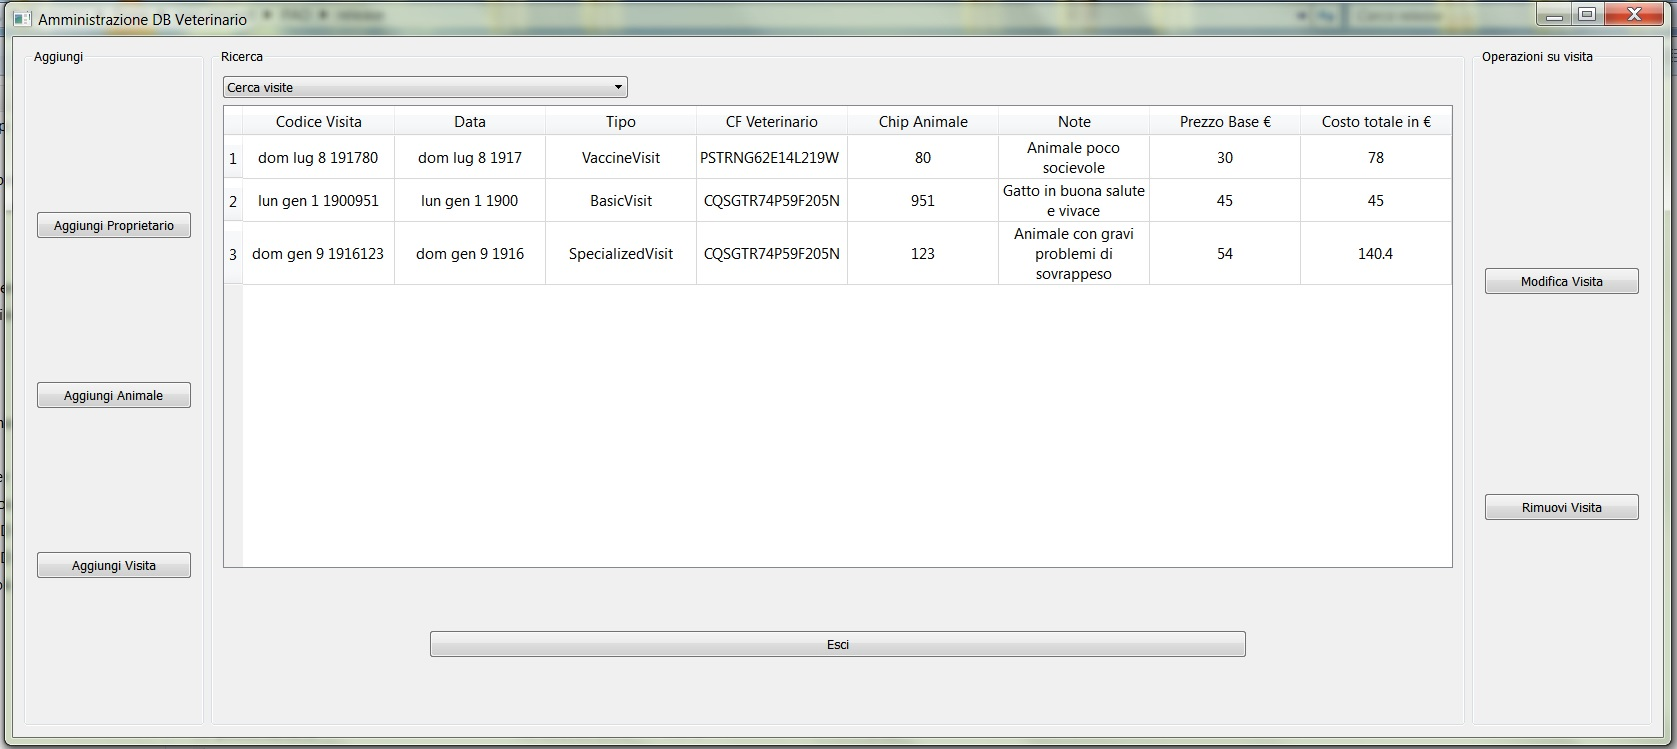
\includegraphics[width=\textwidth]{images/main_view_visits.jpg}
	\caption{La finestra d'amministrazione principale con le visite caricate}
\end{figure}


\begin{figure}
	\centering
	\begin{minipage}{0.45\textwidth}
		\centering
		%\exedout % first figure itself
		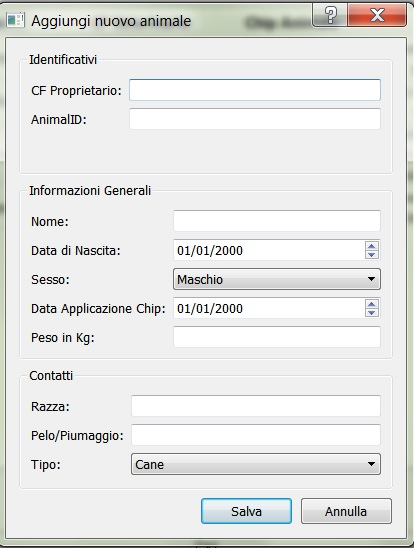
\includegraphics[width=.5\linewidth]{images/addAnimal_view.jpg}
		\caption{Pannello Aggiunta animali}
	\end{minipage}\hfill
	\begin{minipage}{0.45\textwidth}
		\centering
		%\exedout % first figure itself
		\includegraphics[width=.5\linewidth]{images/editvisit_view.jpg}
		\caption{Pannello Modifica Visite}
	\end{minipage}
\end{figure}

\subsection{Nota}
All'inizio la vista è impostata su modalità \textit{Owner} ma la tabella appare vuota. Cambiando il valore della \textit{QComBobox} verranno caricati dinamicamente i dati richiesti.

